\chapter{Design and Implementation}\label{C:workdone}

\section{Overview}

The goal of the project as mentioned in Section \ref{C:intro} is to create a tool to allow developers to identify redundant test cases. The tool can be split into several different sections and each section will be discussed in this chapter. The first objective of the tool was to trace the test data. This involved exploring two different frameworks and comparing the usability of each. After the tool was able to trace the data, we had to determine what spectras we were interested in. The three different spectra types are then discussed. The data that was traced from each test case was then compared to each other to determine the level of redundancy between each test using edit distance metrics. Throughout the testing of the tool, one of the main impediments was the time taken to analysis the large amount of data. We examine how pipelining the output of a heuristic analysis into more computationally heavy analysis decreases the time taken. The final two sections discuss two more advanced areas of the tool. Firstly, retrieving the parameters of the method calls and discussing the trade off parameters create between time taken and more information to analyse. Secondly, giving a weighting to each method call was implemented with the purpose of reducing false positives.

\section{Tracing}
\label{S:trace}
A fundamental requirement for this project was to trace which methods were executed by a test. As David Pearce's language Whiley is written in Java, it was decided to use Java to trace a test. There were two considered tracing frameworks. The first framework considered was AspectJ. The technique that AspectJ uses is called Aspect Oriented Programming (AOP). AOP can be used to add code to an existing program without modifying the source code, this code added is known as an aspect. This process be achieved through the following methods:

\begin{itemize}
\item \textbf{Compile time} --
The classes are compiled with the aspect woven into them. When the program is executed, the methods have the code from the aspect woven into it already. This requires the source to be compiled with AspectJ's compiler.
\item \textbf{Load time} --
The weaving process is deferred until the point at which a class loader attempts to load in a class file. Load time modification is achieved by using a command line argument notifying Java to use the AspectJ class loader.
\end{itemize}

To distinguish what code to weave, and where in the existing code to weave it, a point cut can describe these in AspectJ \cite{aspectj}. The other framework we considered was the Java Debugging Interface (JDI). JDI is similar to using an observer pattern. The list of classes to observe are selected, when a method is called the listening class will be notified if the method has registered to be observed and will be given the information about the method call. 

It was decided to use AspectJ over JDI. AspectJ was easier to choose which methods to record and returns the actual object when retrieving the parameters of the method call. This detail becomes important when we explore tracing parameter values in Section \ref{parameterTrace}. In comparison, JDI was faster to execute, however there was a limited amount of documentation available and the parameters returned were not the actual objects. The decision to use AspectJ was based off this trade off between information and performance. Decoupling the data gathering and data analyse in the tool removed the emphasis on retrieval performance and resulted in the extra information being more important.

To get AspectJ to trace the method details, a point cut was made to record every execution. A simplified version of the aspect is shown in Figure \ref{fig:aspectused}. There are two point cuts within the aspect, the first point cut is going to be called for every method which has a Junit \@Test annotation attached to it. This will then let a static service know that a new test has been started. The second point cut is used to trace everything apart from methods with a  \@Test annotation attached. The next stage was to weave the aspect into the benchmark. Using compile time weaving would have meant that each benchmark needed to be recompiled using the aspect compiler. In contrast, load time only requires the AspectJ class loader to be passed through a command line argument. Load time was chosen for it's ease of use when working with external benchmarks as it only required AspectJ's class loader.

\begin{figure}[h]
\begin{center}
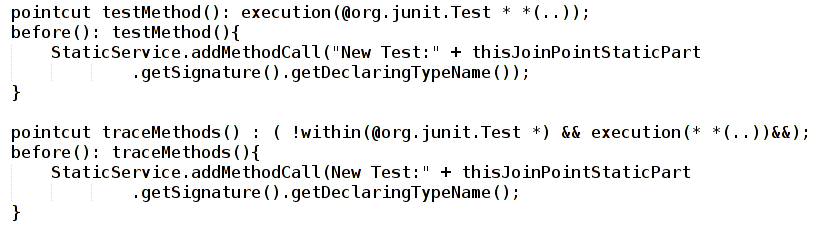
\includegraphics[width = \textwidth]{aspect.png}
\end{center}
\caption{A simplified point cut within AspectJ. The first point cut is for when a new test is executed and the second when a new method is executed.}
\label{fig:aspectused}
\end{figure}

\section{Test Spectra}
\label{S:spectra}
The idea of a spectrum was previously identified in Chapter \ref{C:intro}. Reexamining the idea, a spectrum is some abstraction of the method execution information that is retrievable during the execution of a test. The data retrieved can be split into three different types of spectra, these are \textit{unique method calls}, \textit{every method call} and \textit{calling context}. To explore the different spectra's, an example trace of methods, 'kitten' will be used. Each letter represents a method execution and each letter is executed by the same method. The different spectra's take up different levels of resources. The resources explored are -- time taken and memory. 

\subsection{Unique Method Calls}
The unique method call spectra is where every method execution is only taken into account once. Examining the example trace, the output would be 'kiten', with the difference being the removal of the repeated 't' method. The implication of limiting the method calls to one per method call on the number of comparisons will be dependent the benchmark. Using Whiley Compiler benchmark as an example, there are 494 unique method executions for a single test and 80,000 method calls to these method executions. Utilising the unique method call method, the tool will only compute the redundancy of 494 method executions, rather than the 80,000, $\rfrac{6}{1000}$ of the original amount. The motivation of the spectra is to substantially reduce the time taken and memory used. However, by decreasing the amount of data means that there is a decrease in confidence that the tests produced are redundant test cases. How this fits into the tool is explored in Section \ref{pipelinesection}. \todo{Unsure if this last sentance is good or just to remove}

\subsection{Every Method Call}
The every method call takes into every method execution, analogous to a list of method calls. This spectra is the same as using a calling context of one, where only the highest method execution is examined. Examining the example trace, the output would be 'kitten', with there being no difference between the two. Using the Whiley Compiler benchmark as an example, a list spectra would compute the redundancy of all 80,000 method calls. Comparing this to the unique method call spectra, this is expected to lead to an increase in the time taken but also increase the credibility of the results. 

\subsection{Calling Context}
A calling context contains a separate node for each parent method that the method was called from \cite{Zhuang06accurate}. The number of call retained is referred to as the K depth. The motivation behind the approach is to increase the credibility of the results by taking into account for more data. The consequence of increasing the amount of data is an increase in the time taken and memory used to analyse. Examining the example trace, the output would be 'Parent $\rightarrow$ k, Parent $\rightarrow$ i, Parent $\rightarrow$ t ...). Using the Whiley Compiler benchmark as an example, a calling context spectra would examine all 80,000 method calls, with each containing K depth of method calls. 

To retrieve the calling context in Java, the current stack trace of a method call is examined and then parsed to retrieve the relevant information. This parsing involves removing the method calls that are used to retrieve the stack trace and any memory location details.  \todo{Should i remove this or introduce every section?}In the next section, two different analysis metrics are introduced and examined.

\section{Analysis Metrics}
\label{S:metrics}
The data retrieved from the tracing process needs to be analysed to produce a quantitative value. The value produced will be used to determine the level of similarity between two test cases. Edit distance metrics were discussed in Section \ref{editdistbg}, with two different edit distance metrics considered. They were Monge \& Elkan \cite{monge1997efficient} which splits the strings into sections and compares the sections and Levenshtein \cite{levenshtein1966binary} which compares tokens, generally tokens are single characters. 

For both of the algorithms, there were publicly available frameworks that implemented them. Both implementations allowed for the method calls to be represented with a token. Each test case contained a list of the tokens to represent the trace information of it. The issue with Monge \& Elkan was it attempted to find the best match. Attempting to find the best match would increase the time taken, perform unnecessary computation for our requirements and increase the false positive rate. Using an example of trace information in Figure \ref{fig:mongevleven}. The implementation of Monge \& Elkan would find the best match, in turn matching 'Method Call' in test case 1 to the 'Method Call' in test case 2. Levenshtein did not search for a match, and instead only looked at the opposing method call. This one to one matching was preferred as we were interested in the order of the method calls as well as what methods were called. Overall, Levenshtein integrated better into the tool's ability to identify redundant test cases.

\begin{figure}[h]
\begin{center}
\includegraphics[width = \textwidth]{MongeVLeven.png}
\end{center}
\caption{An example showing how Monge \& Elkan split the method calls into token, where Levenshtein represents the method calls as a whole.}
\label{fig:mongevleven}
\end{figure}

\section{Pipeline}
\label{pipelinesection}
For the tool to help developers reduce the number of redundant tests, it has to analysis the information within an acceptable time frame. By comparing every test with every other while using all of the available information (calling context), this resulted in the analysis taking several days to complete. This is not considered an acceptable time frame. This issue arises when the spectrum's of the test cases contain tens of thousands of method calls. A pipeline approach was implemented which utilised the unique method call spectra as a heuristic. The goal of the pipeline was that each stage should soundly eliminate pairs from consideration that the following stages would have removed. The pipeline approach is shown in Figure \ref{fig:pipeline}. Each analysis stage can be set by the developer within a properties file, these settings are -- the spectra type, analysis metric to use and level of redundancy for each.

To further expand on the heuristic idea. Unique method calls spectra was used as it examined a subset of the available data. Inspecting the subset of data increased the speed of comparison but as a consequence decreased the credibility of our results. The following illustrates an example of this where each character represents a method call.
\paragraph{Comparison 1}
$K,I,T,C,H,E,N$ \& $K,I,B,E,N,Z $
\paragraph{Comparison 2}
$K,I,T,C,H,E,N$ \& $K,I,T,C,H,N$
\paragraph{}
Inspecting comparison 1, it is clear that the two sets of trace information are different. Examining comparison 2, there is a chance that the tests may be redundant so the comparison should be get through the analysing stage and onto the next. Using a benchmark example of Whiley on the wyc package, a heuristic approach enables us to decrease the number of test case comparisons from 90,902 to 100 for the most computationally heavy stage.

The list spectra may also be used as another type of heuristic. The motivation behind the spectra is to use during the second stage in the pipeline to decrease the amount of comparisons that the final pipeline should do. This approach would not be used in the last pipeline as there is limited sense to use a subset of information retrieved from the test cases.

\begin{figure}[h]
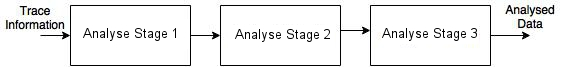
\includegraphics[width=\textwidth]{Pipeline.jpg}
\caption{Trace information goes in at the start of the pipeline. After each stage there should be a reduction of comparisons that the next stage has to complete. The last stage should be the most computationally heavy.}
\label{fig:pipeline}
\end{figure}

\subsection{Saving to the Network}
To execute the analysis on a grid computing system, the test data had to accessible on the School of Engineering's local network. To achieve this, the data retrieved by the tool was saved to the local network. Not only did it allow for the analysis to be executed on the grid system, it also it allowed for the data to be reanalysed without having to re execute the test suite. 

\section{Tracing Parameter Values}
\label{parameterTrace}
The related work in the research area has explored using statement coverage while ignoring the parameter values of each method. It could be argued that due to knowing the statement path, parameters are irrelevant as you know the path the method will take, and parameters do not add any more information. When tracing at method level rather than at the statement, these become crucial to determine the degree of redundancy between test cases. Parameters give insight into the execution paths that will be taken and act as a proxy to the statement information without storing the same amount of the data.

There were two variations of parameters that were considered to trace. Firstly, primitive types only. By running test experiments on the benchmarks, the use of primitives showed that only a limited number of parameters were collected. The parameters collected had a limited effect on the number of false positives identified and time taken. The second approach is to use reflection. Reflection is the ability to examine and modify objects at run time \cite{oraclereflection}. Since AspectJ gives direct access to the object's in the parameters, reflection can be used. By using reflection, the fields of the objects are retrieved and returned in a string to represent the state of the object. This string is then examined to remove any Java object reference location and stored.

The most common use case of the tool is expected to use parameters therefore it was decided to optimize this through storing the data with parameters. The optimization involved saving the parameters with the trace information. If parameters value is set to false, the parameters have to be split off rather than added on. This means that setting the parameters to false would increase the set up time.

\section{Weighting}
Maurer et al. \cite{koochakzadeh2009test} and Robinson et al. \cite{li2008static} found that test suites often had a set of methods that were in every test, such as setup and tear down. These common methods could create false positives. To understand why, a redundant test is one where it is nearly or exactly a replication of another test. Since each method call within a spectra has the same weighting, the more setup and teardown calls made means that the execution stage has decreased weighting overall. We can see an example of this in Figure \ref{fig:weightingdiagram}. The figure shows test cases with different proportions of setup and tear down in relation in the execution stage. The figure also shows how the size of the test case may effect the proportion.

Two different variations of weighting were considered. The first variation involved giving each method execution a weighting based on its call frequency, the higher the frequency, the lower the weighting. This would cause the more common methods to have less impact on the final result, but not be removed completely. The other variation that was considered, and used, was completely removing the most used method calls for each test case. This involved removing every method execution that was more than 80 percent of the most frequent method call. During initial experiments, the first variation was found to have less impact. The reason was that the frequent method calls were still having a large impact, even with a lower weighting. This meant that each benchmark needed different weightings therefore it was difficult to find a solution that could be applied on every benchmark.

Another decision was the scope of the weighting, either it was calculated per test case or test suite. The issue with calculating per suite was that if the benchmark contained a mixture of large and small tests, this could cause the smaller benchmarks to be reduced to a minimal number of method calls. The minimal number of method calls was often not enough information to present the test in a representable state. A per test case weighting was desired to reduce the issue of test cases being reduced to a minimal size.

\begin{figure}[h]
\includegraphics[width=14cm, height=6cm]{weightingdiagram.png}
\caption{A diagram showing how the different size of the test case can be affected by setup and teardown methods.}
\label{fig:weightingdiagram}
\end{figure}